\subsection{A selected command-divergence diagnostic}

Cohort C uses one frozen 250-step direct-scoring checkpoint and one selected episode, evaluated separately from D. At the original 10-ms plant cap, its normal-path delays of 13, 38, and 50~ms yield costs of 0.0362894, 0.0099116, and 0.0366019 with zero misses. Original fallback-path latency is retained. This case accounts for the entire net replay degradation in its nine-normal-episode confirmation group; the other eight episodes slightly offset it. Specifically, the group mean rises from 0.0078931 to 0.0109471, while the other eight means change from 0.0077397 to 0.0077150. The selected case's contribution is 100.719\% of the net increase, not a population frequency.

The first differing requested vector for 13 versus 38~ms occurs at 1.4~s. The 13-ms run chooses $[0.24,0,0.32,0]$, applied at 1.413~s, whereas the 38-ms run chooses $[0.28,0,0.28,0]$, applied at 1.438~s. Their top-two score gaps are 0.02992 and 0.01146. For 50 versus 38~ms, the first difference is at 2.7~s: $[0.32,0.08,0.36,0.32]$ is applied at 2.750~s and $[0.32,0.12,0.36,0.28]$ at 2.738~s. Score gaps are 0.02205 and 0.000711.

At both first divergences, the admission masks match, the filter does not intervene, and the chosen candidates remain approximately 47.15 and 45.99~K below the calibrated gate threshold. Thus, a score-ordering change identifies the first differing request, with no active gate boundary at that point. Figure~\ref{fig:divergence} shows individual applied heater commands. The request-aligned mean of requested command vectors first differs at 4.5~s, concealing the earlier redistribution between heaters. Actual applied-command means differ earlier because application times already differ. Scores are model outputs, so their small gaps do not quantify thermal or integration error.

\begin{figure}[tbp]
\centering
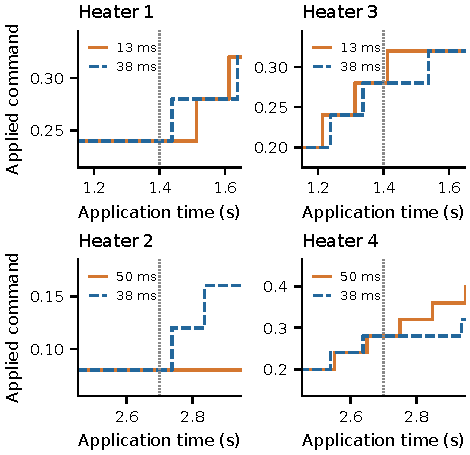
\includegraphics[width=\linewidth]{figures/first_command_divergence.pdf}
\caption{Individual applied commands around the first differing requested vectors in cohort C. Upper panels compare 13 and 38~ms near the 1.4-s request; lower panels compare 50 and 38~ms near 2.7~s. Dotted lines mark request times; steps use actual application timestamps.}
\label{fig:divergence}
\end{figure}

Recomputing the decisions at smaller plant steps changes this case substantially. The lowest-cost normal-path delay changes from 38 to 50 to 13~ms as $\Delta t_{\max}$ decreases from 10 to 5 to 2.5~ms. For the 13-ms condition, the cost falls from 0.0369141 at 5~ms to 0.0091314 at 2.5~ms, a 75.26\% change. All nine closed-loop recomputations complete without deadline misses. The original 38-ms advantage therefore does not persist under numerical refinement.

\begin{figure}[tbp]
\centering
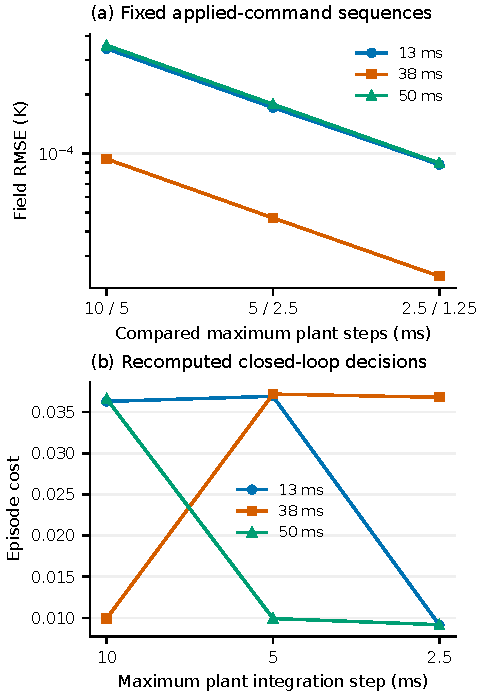
\includegraphics[width=\linewidth]{figures/numerical_case_C.pdf}
\caption{Numerical sensitivity of the selected C episode. (a) Temperature-field RMSE between successive plant-step refinements, sampled at 1~Hz, with each original applied-command sequence fixed. (b) Closed-loop costs when decisions are recomputed at each plant cap. The three colors identify the normal-path delay conditions.}
\label{fig:numericalC}
\end{figure}

Holding each original applied-command sequence fixed produces much smaller differences. From 10 to 1.25~ms, the absolute relative cost change stays below 0.0032\% for all three sequences. Across the 1-Hz full-field samples, the largest trajectory RMSE is $6.25\times10^{-4}$~K and the largest pointwise difference is $3.62\times10^{-3}$~K. Differences between successive refinements approximately halve (Fig.~\ref{fig:numericalC}). These are observed differences between finite resolutions, not bounds on the continuous-time solution.

The small fixed-input changes and large closed-loop changes are consistent with amplification through observation-dependent, discrete candidate choices and subsequent feedback. They do not identify a unique numerical mechanism or establish an optimal physical delay. C remains a supporting sensitivity diagnostic; the stable aggregate comparisons in D concern different frozen residual systems.

